%---------------spy effect----------------------
\newif\ifblackandwhitecycle
\gdef\patternnumber{0}

\pgfkeys{/tikz/.cd,
    zoombox paths/.style={
        draw=orange,
        very thick
    },
    black and white/.is choice,
    black and white/.default=static,
    black and white/static/.style={ 
        draw=white,   
        zoombox paths/.append style={
            draw=white,
            postaction={
                draw=black,
                loosely dashed
            }
        }
    },
    black and white/static/.code={
        \gdef\patternnumber{1}
    },
    black and white/cycle/.code={
        \blackandwhitecycletrue
        \gdef\patternnumber{1}
    },
    black and white pattern/.is choice,
    black and white pattern/0/.style={},
    black and white pattern/1/.style={    
            draw=white,
            postaction={
                draw=black,
                dash pattern=on 2pt off 2pt
            }
    },
    black and white pattern/2/.style={    
            draw=white,
            postaction={
                draw=black,
                dash pattern=on 4pt off 4pt
            }
    },
    black and white pattern/3/.style={    
            draw=white,
            postaction={
                draw=black,
                dash pattern=on 4pt off 4pt on 1pt off 4pt
            }
    },
    black and white pattern/4/.style={    
            draw=white,
            postaction={
                draw=black,
                dash pattern=on 4pt off 2pt on 2 pt off 2pt on 2 pt off 2pt
            }
    },
    zoomboxarray inner gap/.initial=5pt,
    zoomboxarray columns/.initial=2,
    zoomboxarray rows/.initial=2,
    subfigurename/.initial={},
    figurename/.initial={zoombox},
    zoomboxarray/.style={
        execute at begin picture={
            \begin{scope}[
                spy using outlines={%
                    zoombox paths,
                    width=\imagewidth / \pgfkeysvalueof{/tikz/zoomboxarray columns} - (\pgfkeysvalueof{/tikz/zoomboxarray columns} - 1) / \pgfkeysvalueof{/tikz/zoomboxarray columns} * \pgfkeysvalueof{/tikz/zoomboxarray inner gap} -\pgflinewidth,
                    height=\imageheight / \pgfkeysvalueof{/tikz/zoomboxarray rows} - (\pgfkeysvalueof{/tikz/zoomboxarray rows} - 1) / \pgfkeysvalueof{/tikz/zoomboxarray rows} * \pgfkeysvalueof{/tikz/zoomboxarray inner gap}-\pgflinewidth,
                    magnification=3,
                    every spy on node/.style={
                        zoombox paths
                    },
                    every spy in node/.style={
                        zoombox paths
                    }
                }
            ]
        },
        execute at end picture={
            \end{scope}
             \node at (image.north) [anchor=north,inner sep=0pt] {\subcaptionbox{\label{\pgfkeysvalueof{/tikz/figurename}-image}}{\phantomimage}};
              \node at (zoomboxes container.north) [anchor=north,inner sep=0pt] {\subcaptionbox{\label{\pgfkeysvalueof{/tikz/figurename}-zoom}}{\phantomimage}};
     \gdef\patternnumber{0}
        },
        spymargin/.initial=0.5em,
        zoomboxes xshift/.initial=1,
        zoomboxes right/.code=\pgfkeys{/tikz/zoomboxes xshift=1},
        zoomboxes left/.code=\pgfkeys{/tikz/zoomboxes xshift=-1},
        zoomboxes yshift/.initial=0,
        zoomboxes above/.code={
            \pgfkeys{/tikz/zoomboxes yshift=1},
            \pgfkeys{/tikz/zoomboxes xshift=0}
        },
        zoomboxes below/.code={
            \pgfkeys{/tikz/zoomboxes yshift=-1},
            \pgfkeys{/tikz/zoomboxes xshift=0}
        },
        caption margin/.initial=4ex,
    },
    adjust caption spacing/.code={},
    image container/.style={
        inner sep=0pt,
        at=(image.north),
        anchor=north,
        adjust caption spacing
    },
    zoomboxes container/.style={
        inner sep=0pt,
        at=(image.north),
        anchor=north,
        name=zoomboxes container,
        xshift=\pgfkeysvalueof{/tikz/zoomboxes xshift}*(\imagewidth+\pgfkeysvalueof{/tikz/spymargin}),
        yshift=\pgfkeysvalueof{/tikz/zoomboxes yshift}*(\imageheight+\pgfkeysvalueof{/tikz/spymargin}+\pgfkeysvalueof{/tikz/caption margin}),
        adjust caption spacing
    },
    calculate dimensions/.code={
        \pgfpointdiff{\pgfpointanchor{image}{south west} }{\pgfpointanchor{image}{north east} }
        \pgfgetlastxy{\imagewidth}{\imageheight}
        \global\let\imagewidth=\imagewidth
        \global\let\imageheight=\imageheight
        \gdef\columncount{1}
        \gdef\rowcount{1}
        \gdef\zoomboxcount{1}
    },
    image node/.style={
        inner sep=0pt,
        name=image,
        anchor=south west,
        append after command={
            [calculate dimensions]
            node [image container,subfigurename=\pgfkeysvalueof{/tikz/figurename}-image] {\phantomimage}
            node [zoomboxes container,subfigurename=\pgfkeysvalueof{/tikz/figurename}-zoom] {\phantomimage}
        }
    },
    color code/.style={
        zoombox paths/.append style={draw=#1}
    },
    connect zoomboxes/.style={
    spy connection path={\draw[draw=none,zoombox paths] (tikzspyonnode) -- (tikzspyinnode);}
    },
    help grid code/.code={
        \begin{scope}[
                x={(image.south east)},
                y={(image.north west)},
                font=\footnotesize,
                help lines,
                overlay
            ]
            \foreach \x in {0,1,...,9} { 
                \draw(\x/10,0) -- (\x/10,1);
                \node [anchor=north] at (\x/10,0) {0.\x};
            }
            \foreach \y in {0,1,...,9} {
                \draw(0,\y/10) -- (1,\y/10);                        \node [anchor=east] at (0,\y/10) {0.\y};
            }
        \end{scope}    
    },
    help grid/.style={
        append after command={
            [help grid code]
        }
    },
}

\newcommand\phantomimage{%
    \phantom{%
        \rule{\imagewidth}{\imageheight}%
    }%
}
\newcommand\zoombox[2][]{
    \begin{scope}[zoombox paths]
        \pgfmathsetmacro\xpos{
            (\columncount-1)*(\imagewidth / \pgfkeysvalueof{/tikz/zoomboxarray columns} + \pgfkeysvalueof{/tikz/zoomboxarray inner gap} / \pgfkeysvalueof{/tikz/zoomboxarray columns} ) + \pgflinewidth
        }
        \pgfmathsetmacro\ypos{
            (\rowcount-1)*( \imageheight / \pgfkeysvalueof{/tikz/zoomboxarray rows} + \pgfkeysvalueof{/tikz/zoomboxarray inner gap} / \pgfkeysvalueof{/tikz/zoomboxarray rows} ) + 0.5*\pgflinewidth
        }
        \edef\dospy{\noexpand\spy [
            #1,
            zoombox paths/.append style={
                black and white pattern=\patternnumber
            },
            every spy on node/.append style={#1},
            x=\imagewidth,
            y=\imageheight
        ] on (#2) in node [anchor=north west] at ($(zoomboxes container.north west)+(\xpos pt,-\ypos pt)$);}
        \dospy
        \pgfmathtruncatemacro\pgfmathresult{ifthenelse(\columncount==\pgfkeysvalueof{/tikz/zoomboxarray columns},\rowcount+1,\rowcount)}
        \global\let\rowcount=\pgfmathresult
        \pgfmathtruncatemacro\pgfmathresult{ifthenelse(\columncount==\pgfkeysvalueof{/tikz/zoomboxarray columns},1,\columncount+1)}
        \global\let\columncount=\pgfmathresult
        \ifblackandwhitecycle
            \pgfmathtruncatemacro{\newpatternnumber}{\patternnumber+1}
            \global\edef\patternnumber{\newpatternnumber}
        \fi
    \end{scope}
}
%---------------spy effect---------------------------


\chapter{Fundamentals}
\label{ch:basic}


\section{Definition}
UAV is known as the acronyms for ``Unmanned Aerial Vehicle’’ (UAV), which is the most commonly used term in the geomatics community. Besides, there are also other popular terms such as ``drone", ``Micro Aerial Vehicles (MAV)", ``Remotely Piloted Vehicle (RPV)" and ``Remotely-Piloted Aerial System’’ (RPAS). According to their size, payload and weight, UAVs can be divided into three main categories \cite{blyenburgh2013yearbook}: 
\begin{itemize}
\item \textit{tactical UAVs}, which are usually equipped with high-performance avionics and generally used for military applications.
\item \textit{close-short-medium-range UAVs}, whose maximum take-off weight ranges from 150 to 1250 kg with an operative range from 10 km to 70 km.  
\item \textit{nano-micro-mini UAVs}, which is featured by small payload sizes and low weights, generally with an endurance of less than two hours and an operating range of less than 10 km.
\end{itemize}


In this paper, we will refer to UAV as the category of micro unmanned aerial vehicles whose weight is generally less than 5 kg. And the term ``aerial imagery" or ``airborne imagery" specifically refers to the imagery collected by conventional manned aircrafts. An example of typical UAV and aerial platforms is illustrated in Figure \ref{fig:platforms} (a) and (b) respectively.

\begin{figure}[ht!]
    \centering
    \begin{subfigure}{.49\textwidth }
	\centering
        \includegraphics[width=0.9\linewidth]{uav.jpg}
        \caption{AscTec Falcon 8 octocopter}
    \end{subfigure}%\hskip2em
    \begin{subfigure}{.49\textwidth}
	\centering
        \includegraphics[width=0.9\linewidth]{aerial.jpg}
        \caption{DLR’s BO 105 research helicopter.}
    \end{subfigure}
\caption{Typical UAV and airborne platforms used in this paper}
\label{fig:platforms}
\end{figure}

\section{Characteristics}

Recent years have witnessed the fast development of UAVs. As a novel data acquisition platform, UAV bridges the gap between traditional airborne photogrammetry and terrestrial photogrammetry and demonstrates various advantages. Table \ref{tab:comp_charact} compares the main properties of UAV and traditional airborne platforms. With lower flight altitude, UAV imagery presents higher spatial resolution (approximately 1 cm/pixel) in contrast with imagery collected by traditional manned aircrafts (on the order of 25 cm/pixel), offering richer details of the scenes. Besides, conventional aerial photography platforms usually require big landing fields and pilots, and the flight plan is limited by air traffic and the weather. By contrast, UAVs only need small landing sites and can be remotely controlled, therefore they can work in severe weather conditions and even in hazardous areas with lower cost. In long term, UAVs offer superior temporal resolution as UAV-based survey tasks can be frequently updated according to users' demands, which is unpractical for manned aircrafts.
\begin{table}[H]
  \begin{center}
  %\footnotesize 
  \small
  \begin{tabular}{@{}p{.32\linewidth}p{.31\linewidth}p{.31\linewidth}@{}}
    \toprule
    {} & {\textbf{UAV platforms}} & {\textbf{Airborne platforms}} \\
    \cmidrule(){1-3}
    % %
    Spatial resolution/GSD& $cm$ & $dm$ \\
    \midrule
    Flexibility & Total & Flight plan needed\\&&weather dependent\\
    \midrule
    Update frequency & Ad-hoc & No or low\\
    \midrule
    % %
    System cost & $10 \sim1000$ k\euro{} & $1000\sim 10\,000$ k\euro{}\\ 
    \midrule
    Coverage & $\le 1 km^{2}$ & $10 \sim 10\,000km^{2}$ \\
    \midrule
    % %
    onborad GNSS/IMU accuracy & $m$ &$cm$\\
    \bottomrule
  \end{tabular}
  \end{center}
  \caption {Characteristics of UAV and traditional airborne platforms \cite{everaerts2008unmanned}}
\label{tab:comp_charact}
\end{table}


\begin{figure}[ht]\centering
 \begin{subfigure}{0.99\columnwidth}
\begin{tikzpicture}[
    zoomboxarray
]
    \node [image node] {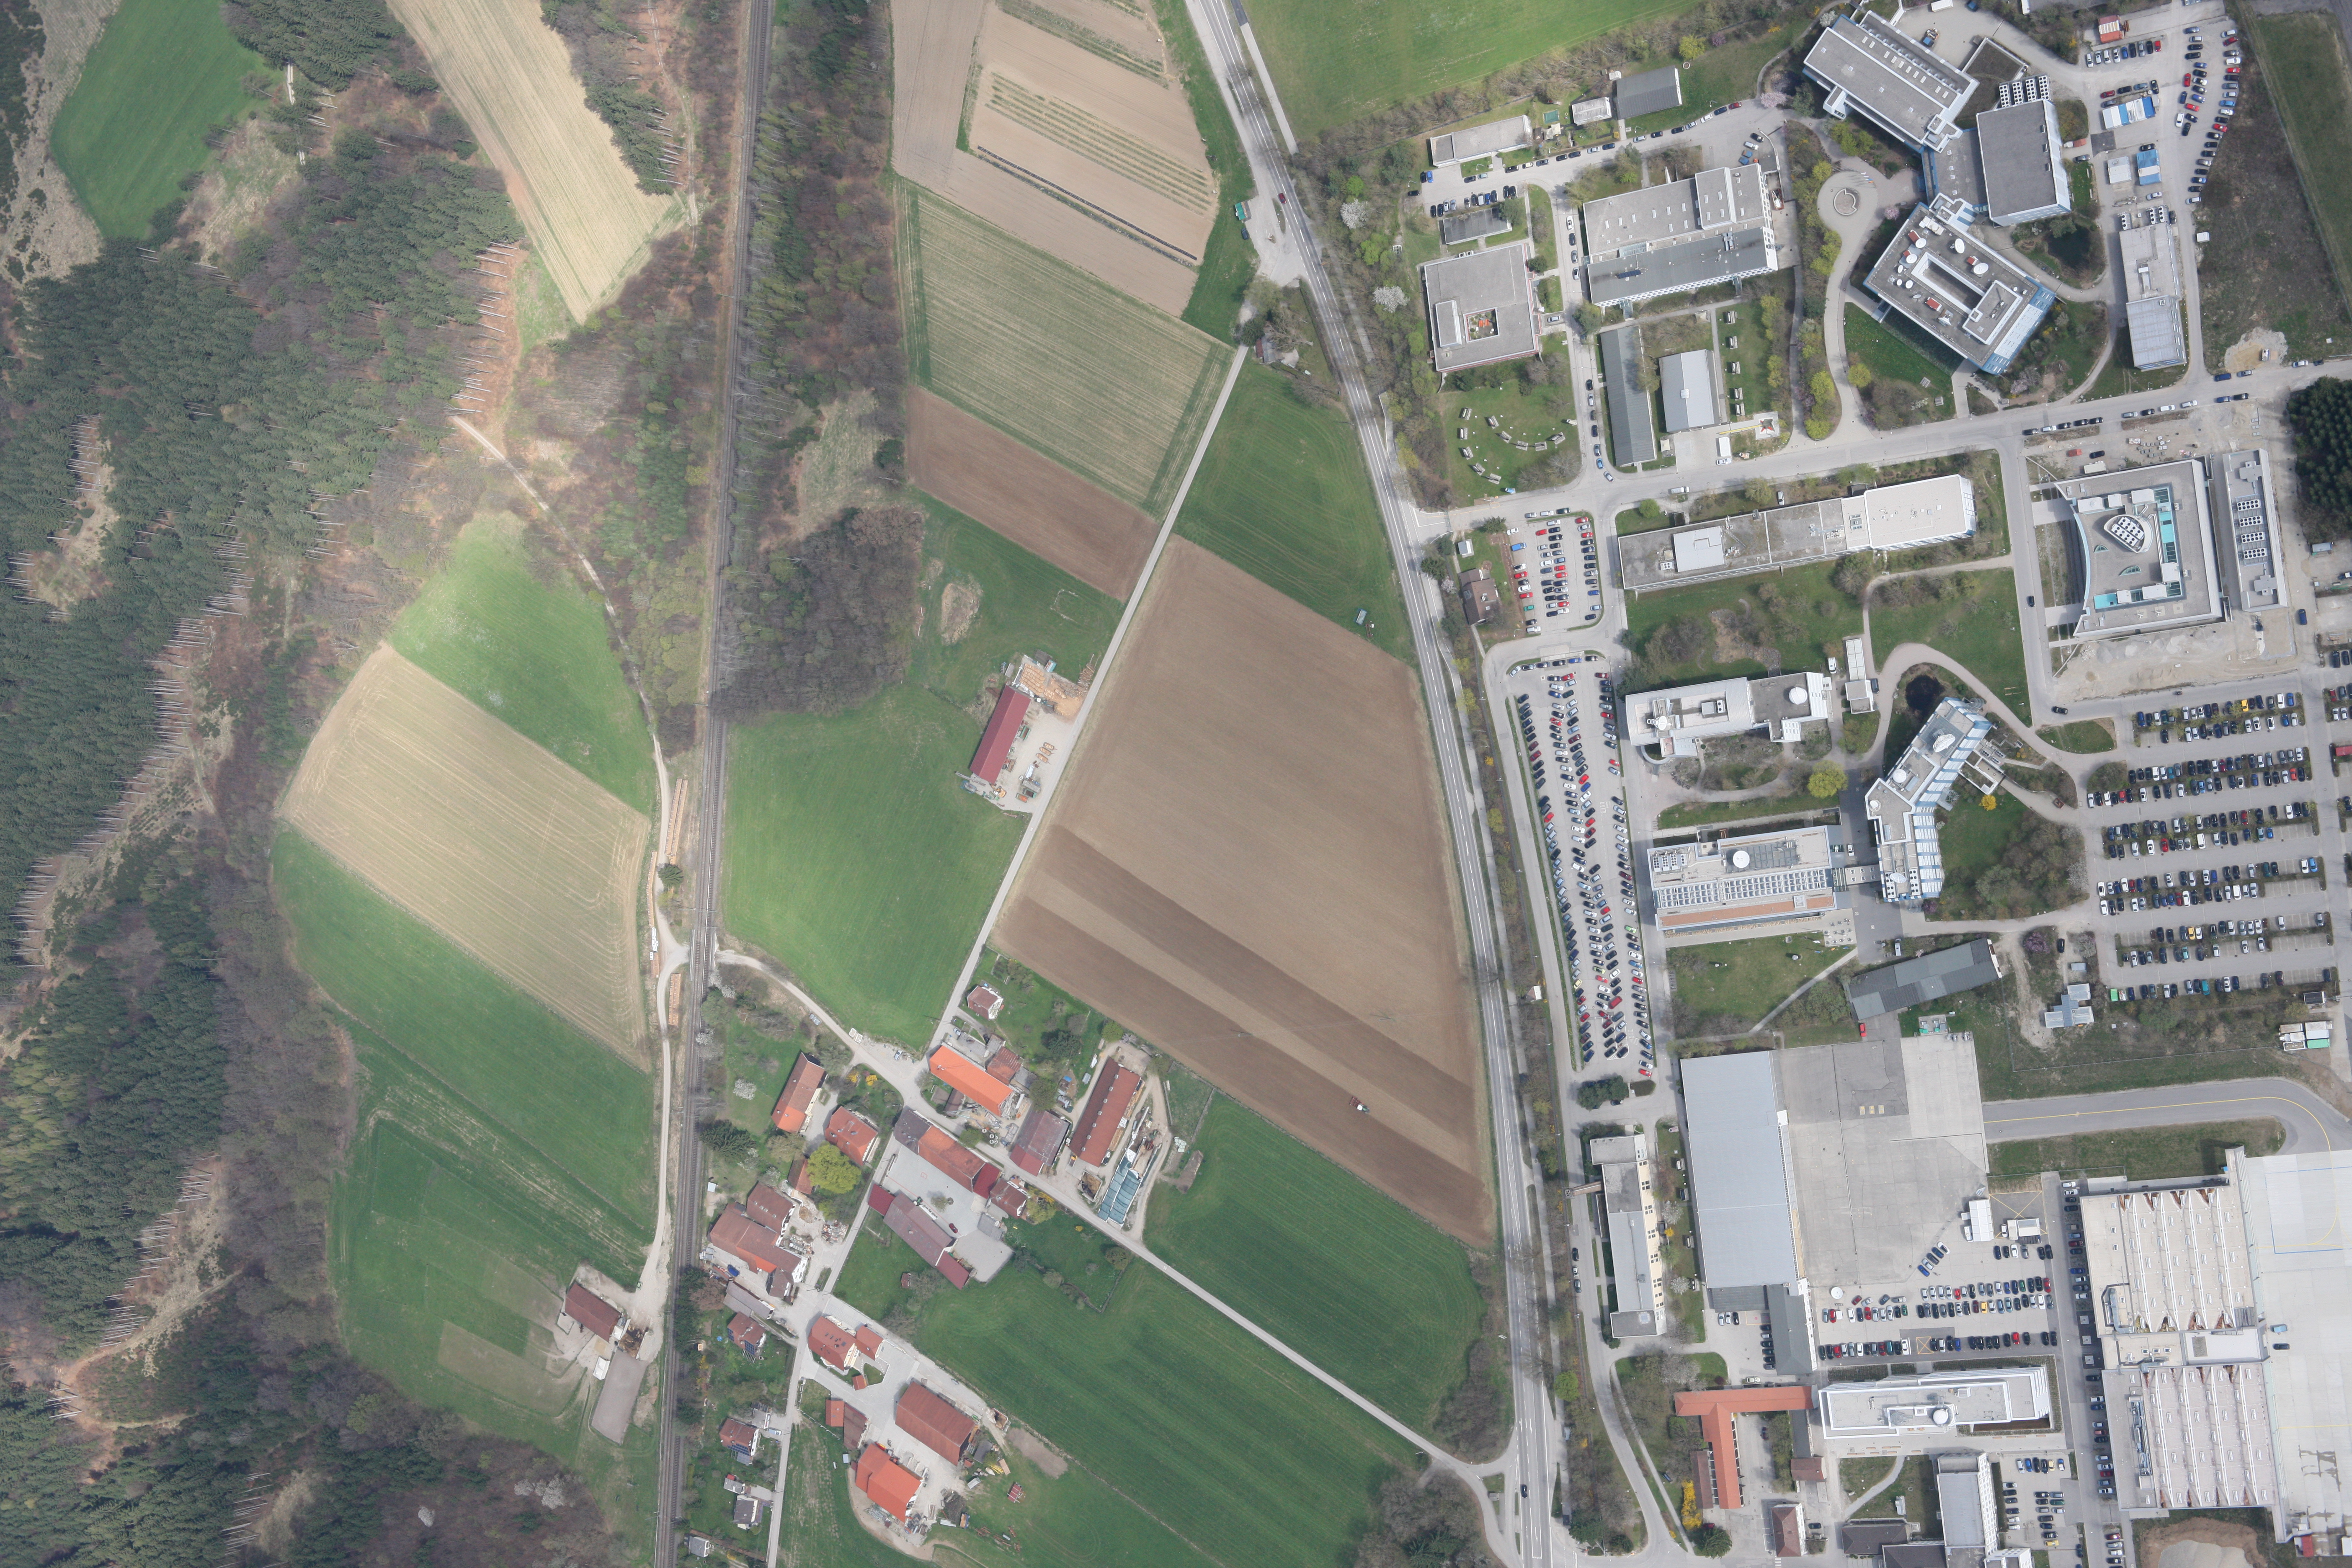
\includegraphics[width=0.5\textwidth]{EK7P0089}};
    \zoombox[magnification=7,color code=yellow]{0.68,0.43}
    \zoombox[magnification=7,color code=red]{0.79,0.44}
    \zoombox[magnification=12,color code=blue]{0.63,0.62}
    \zoombox[magnification=12,color code=green]{0.62,0.7}
\end{tikzpicture} 
 \end{subfigure}

 \begin{subfigure}{0.244\columnwidth}
   \centering
\begin{tikzpicture}
   \centering
    \node[inner sep=0pt] (ima) at (0,0) {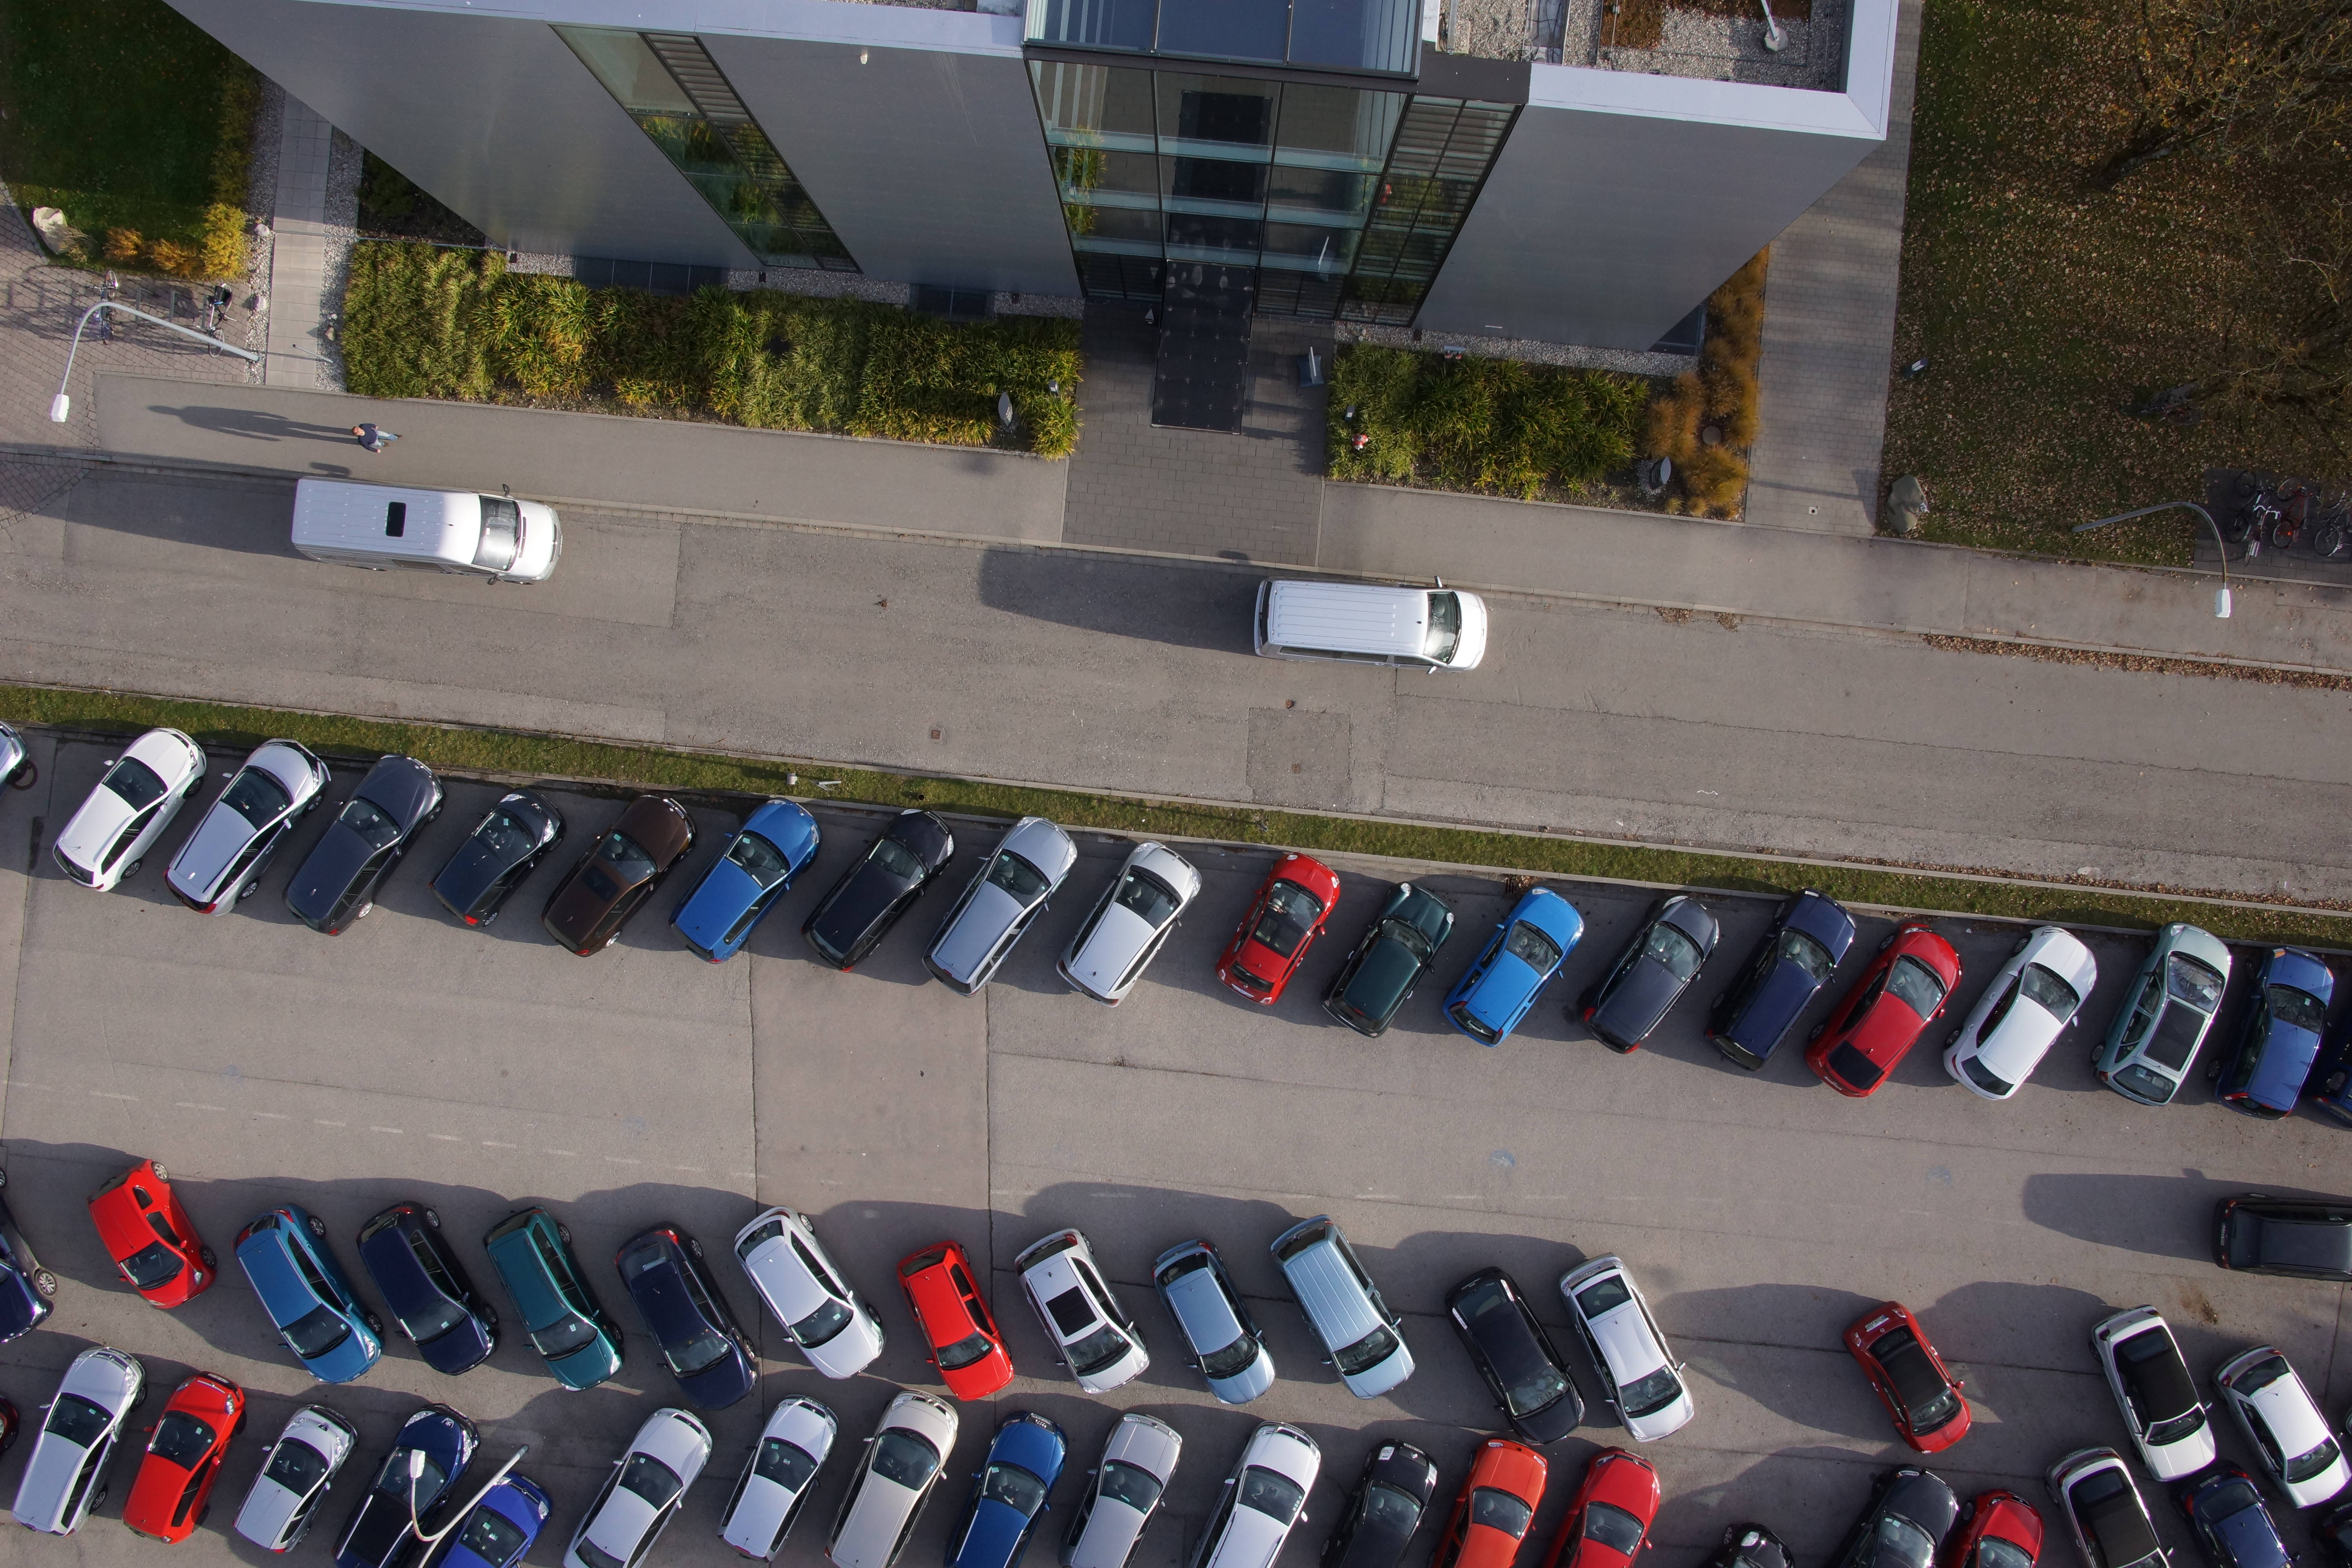
\includegraphics[cfbox=yellow,width=1\columnwidth]{G0000786}};    
 \end{tikzpicture}
 \end{subfigure}
  \begin{subfigure}{0.244\columnwidth}
   \centering
\begin{tikzpicture}
   \centering
    \node[inner sep=0pt] (ima) at (0,0) {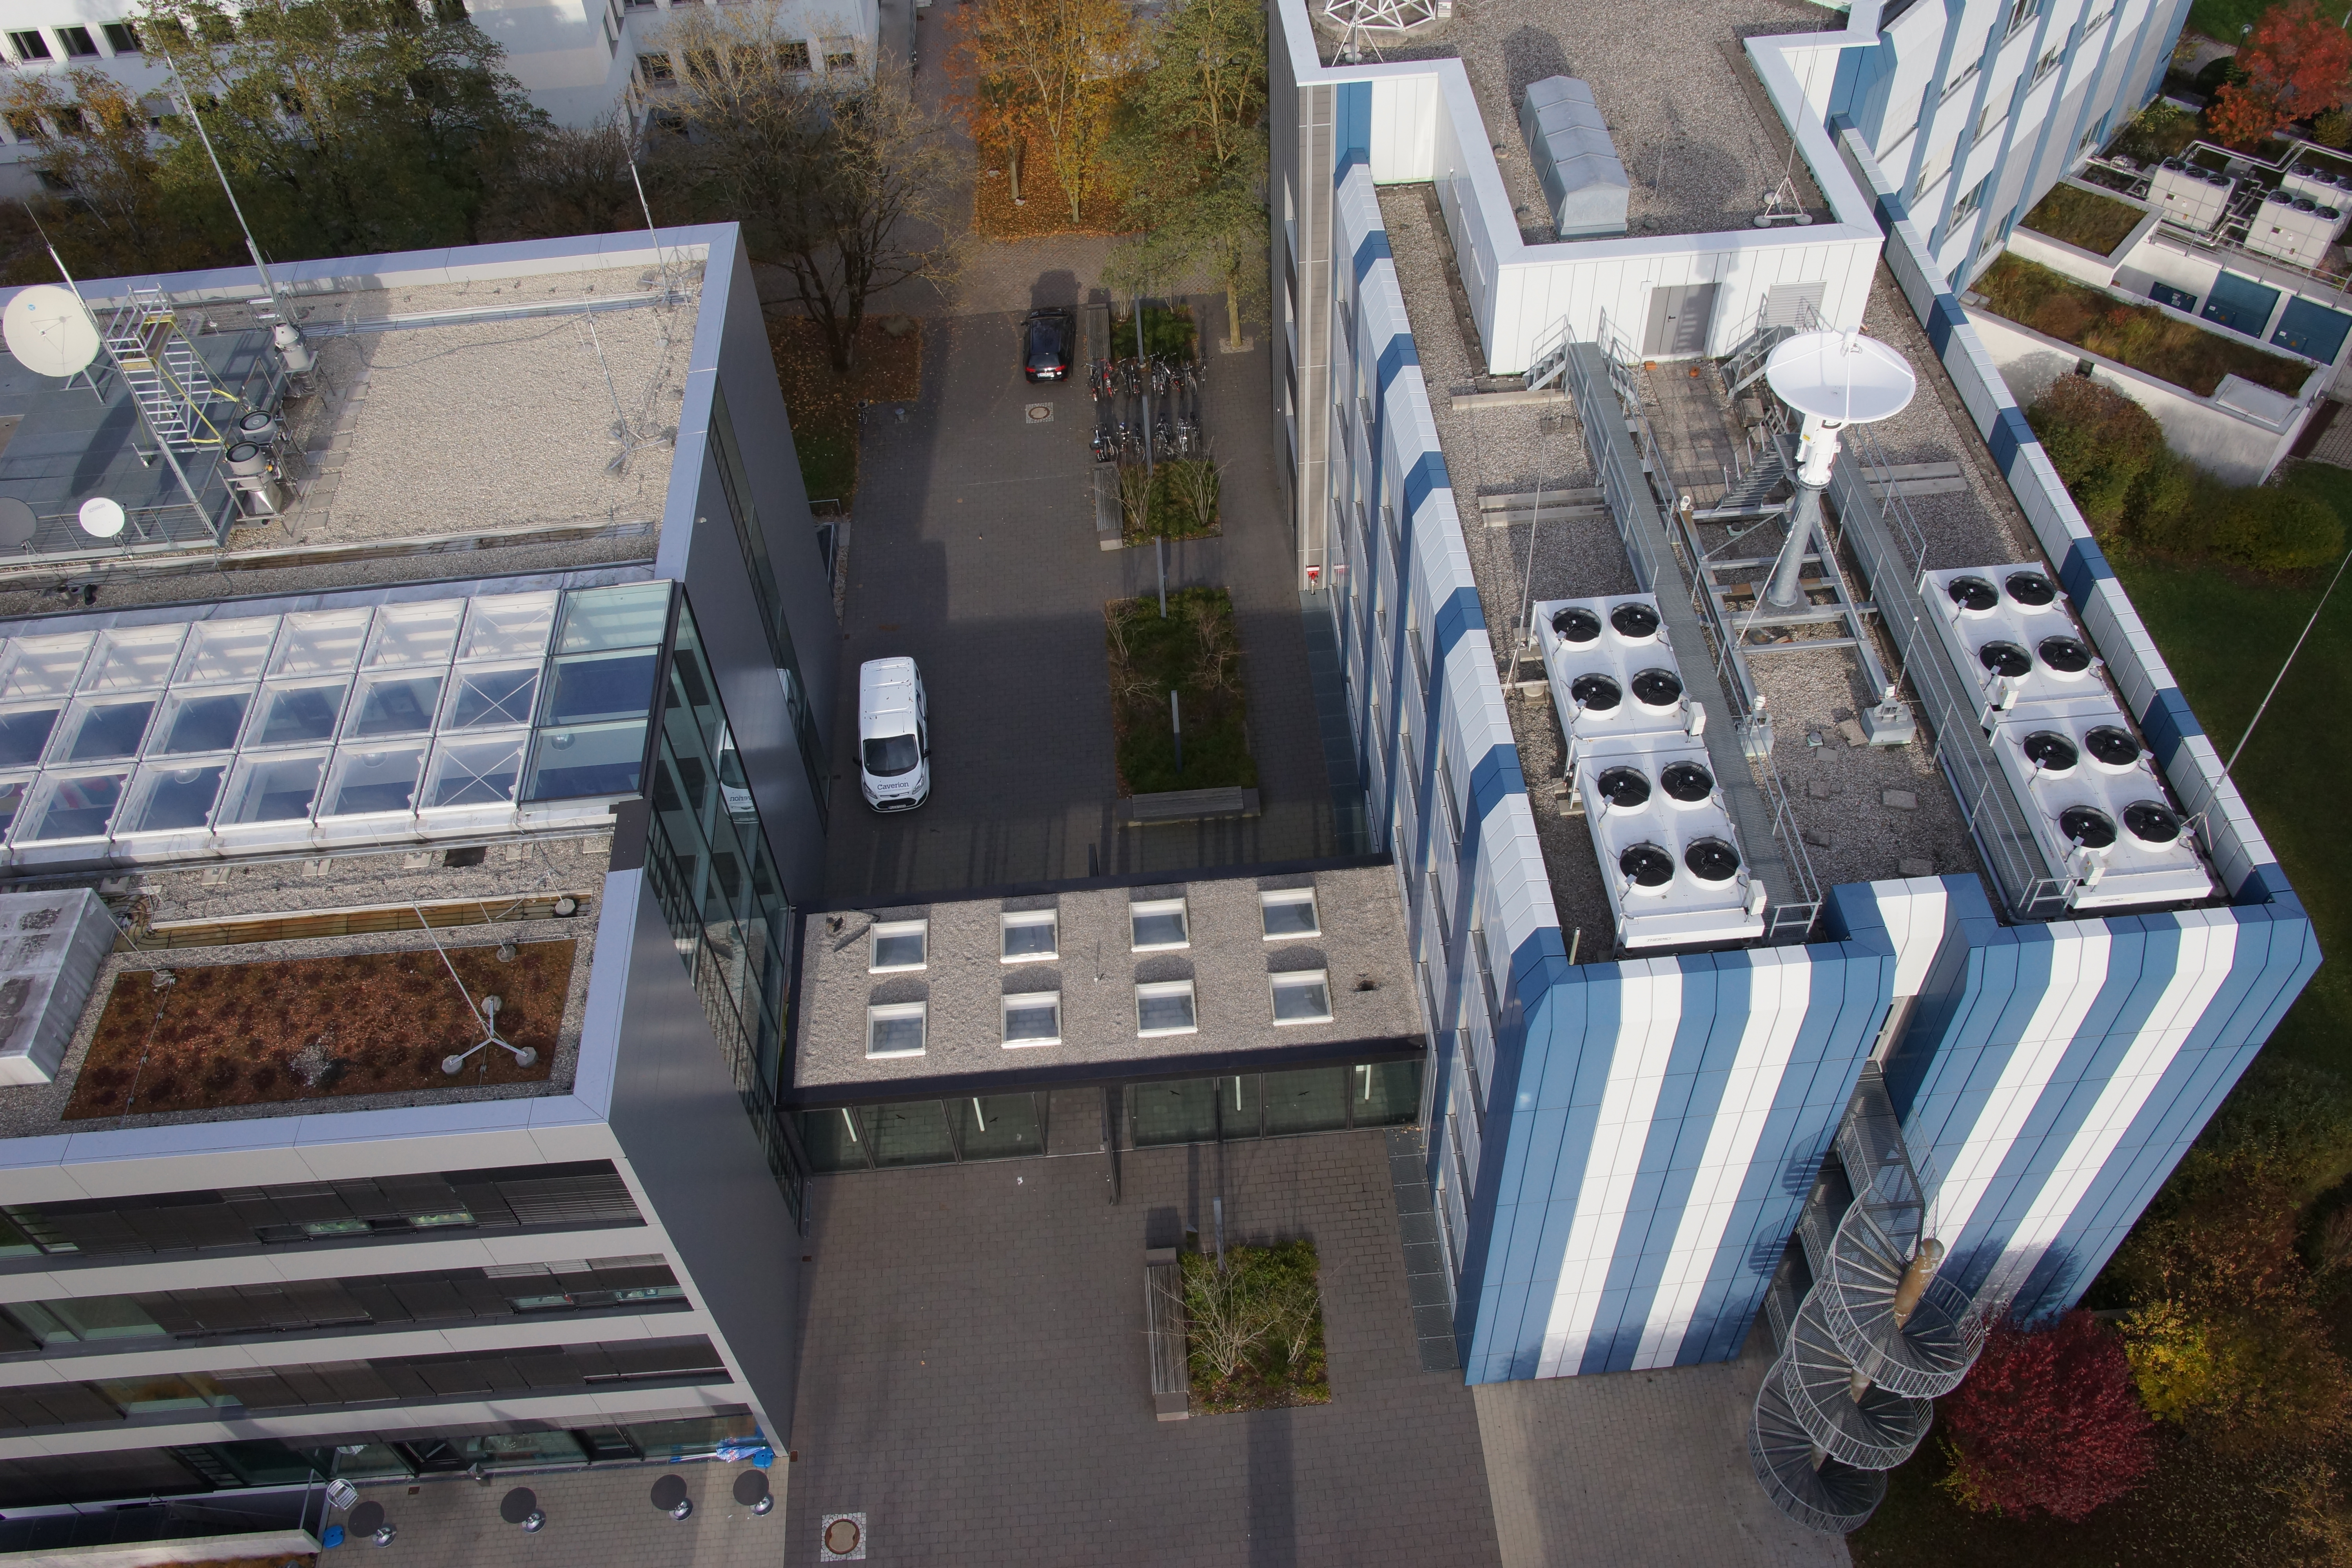
\includegraphics[cfbox=red,width=1\columnwidth]{G0000852}};    
 \end{tikzpicture}
 \end{subfigure}
  \begin{subfigure}{0.244\columnwidth}
   \centering
\begin{tikzpicture}
   \centering
    \node[inner sep=0pt] (ima) at (0,0) {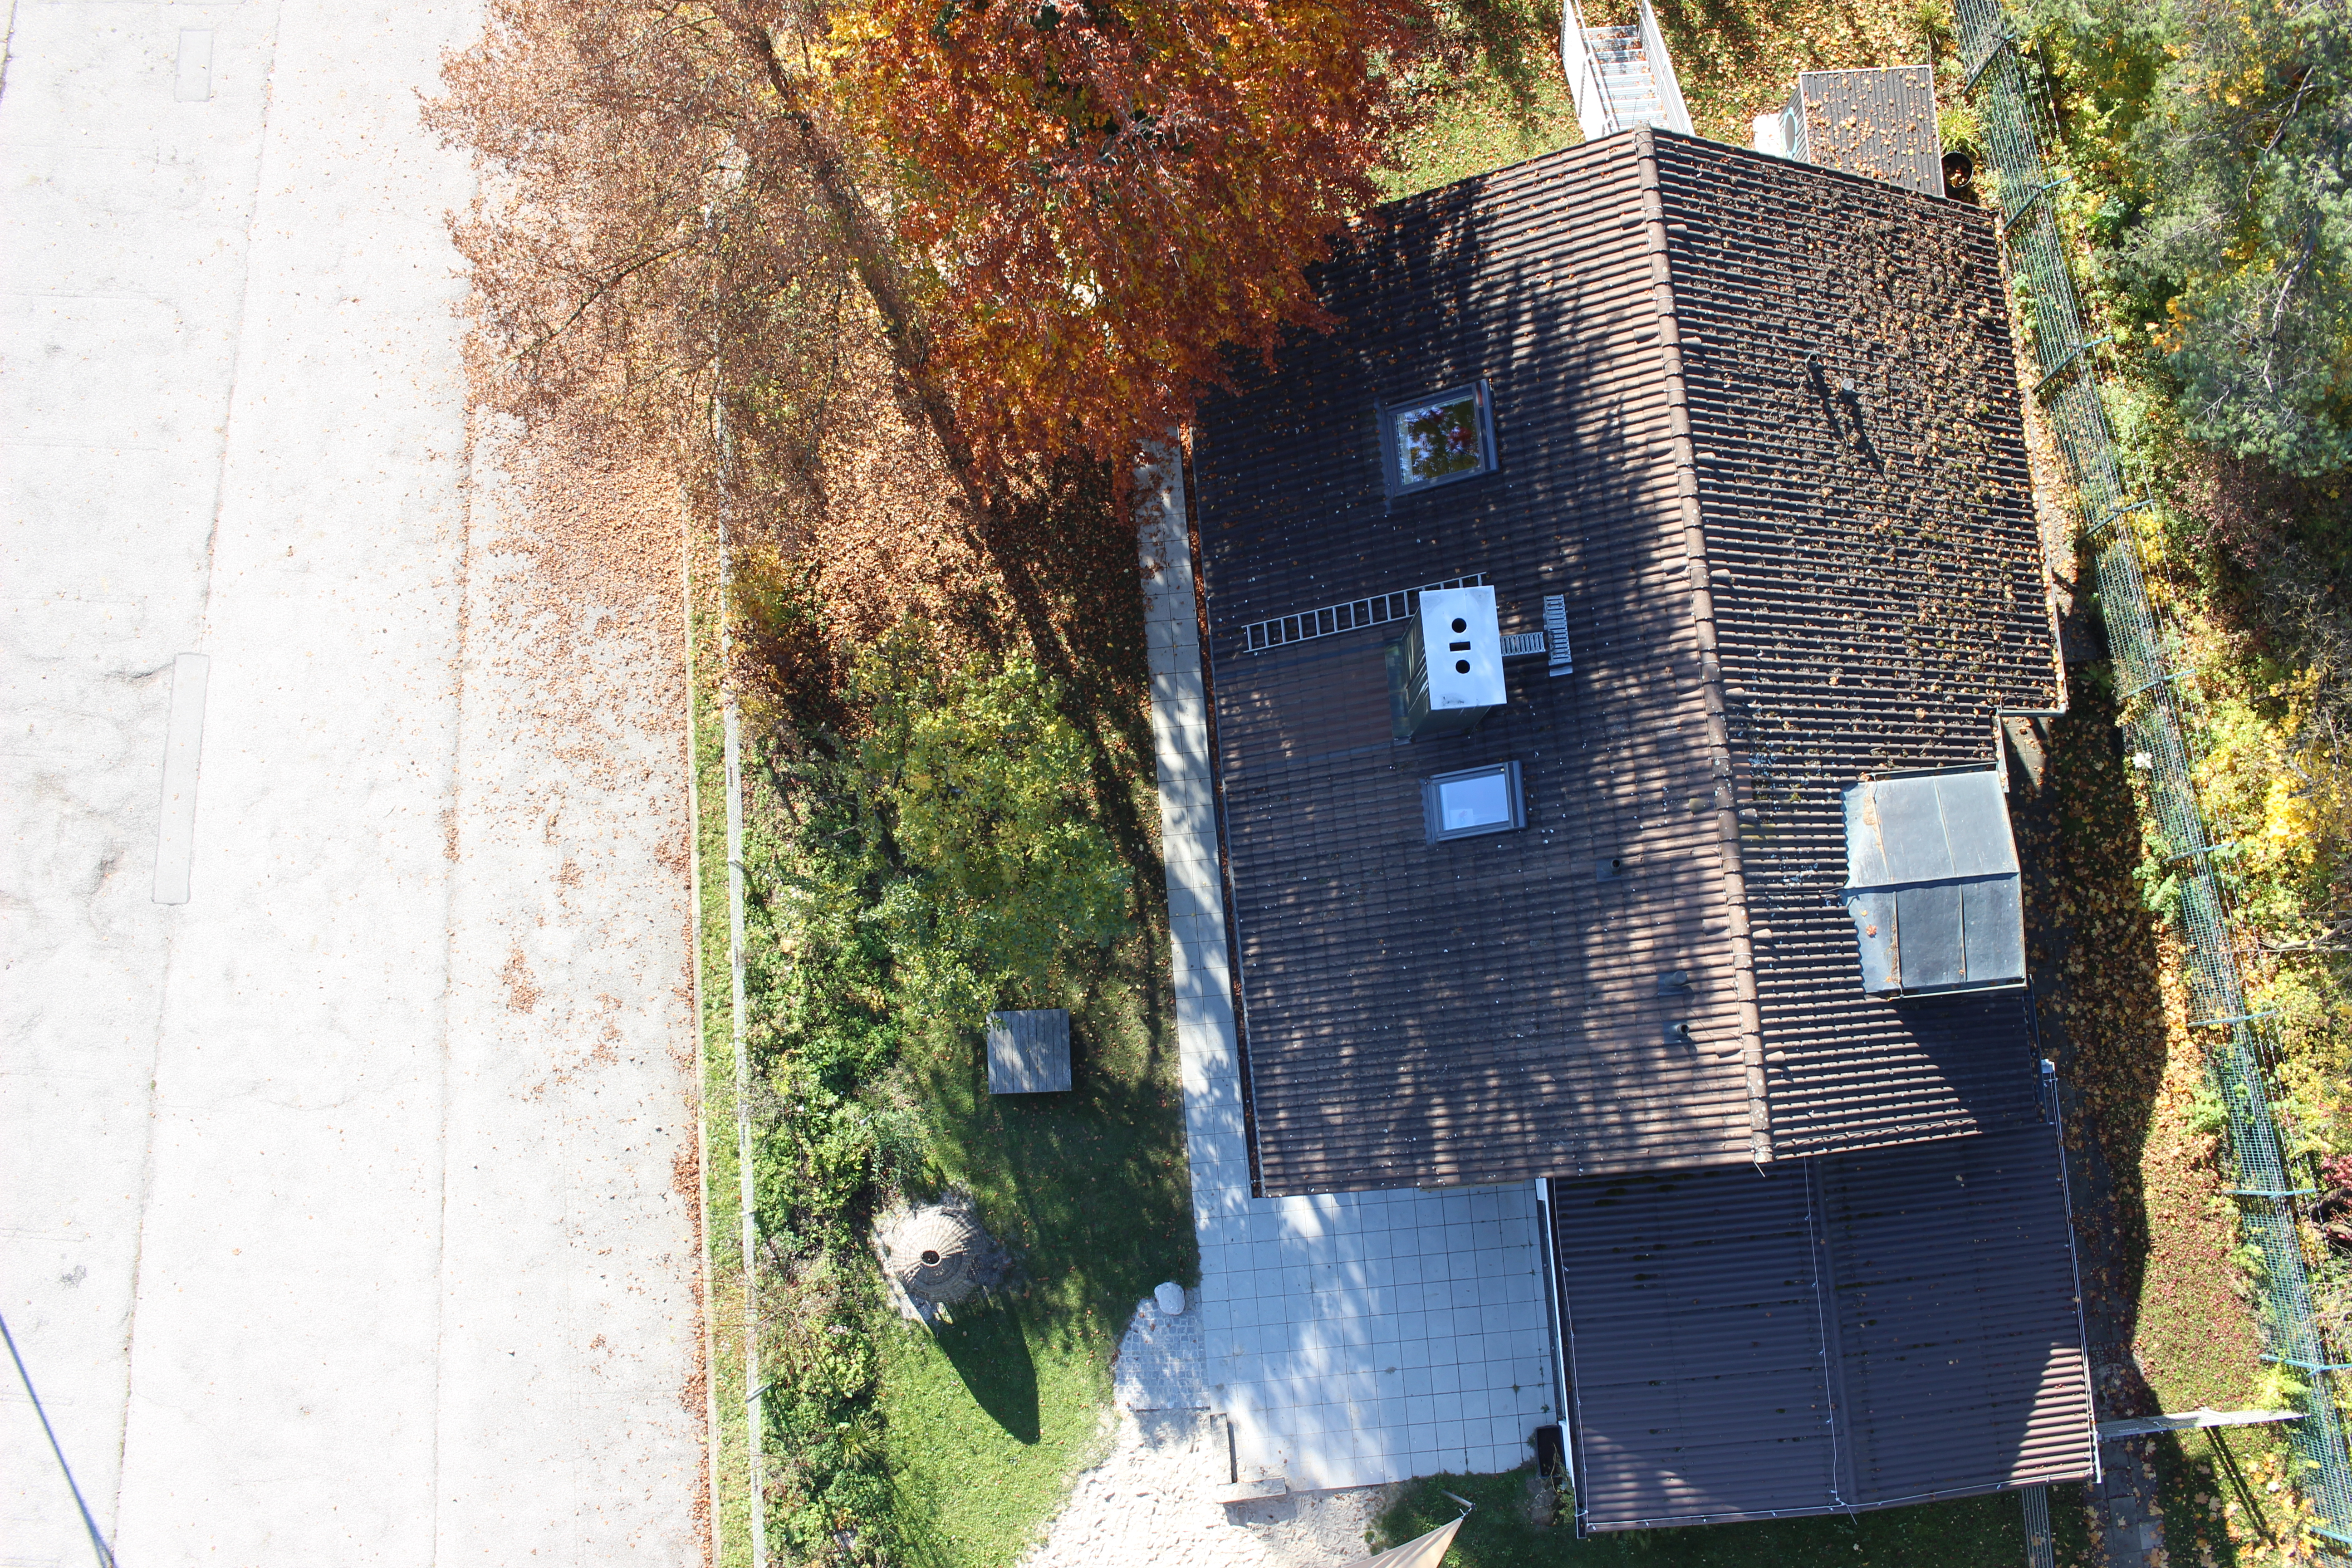
\includegraphics[cfbox=blue,angle=180,width=1\columnwidth]{IMG_1312}};    
 \end{tikzpicture}
 \end{subfigure}
  \begin{subfigure}{0.244\columnwidth}
   \centering
\begin{tikzpicture}
   \centering
    \node[inner sep=0pt] (ima) at (0,0) {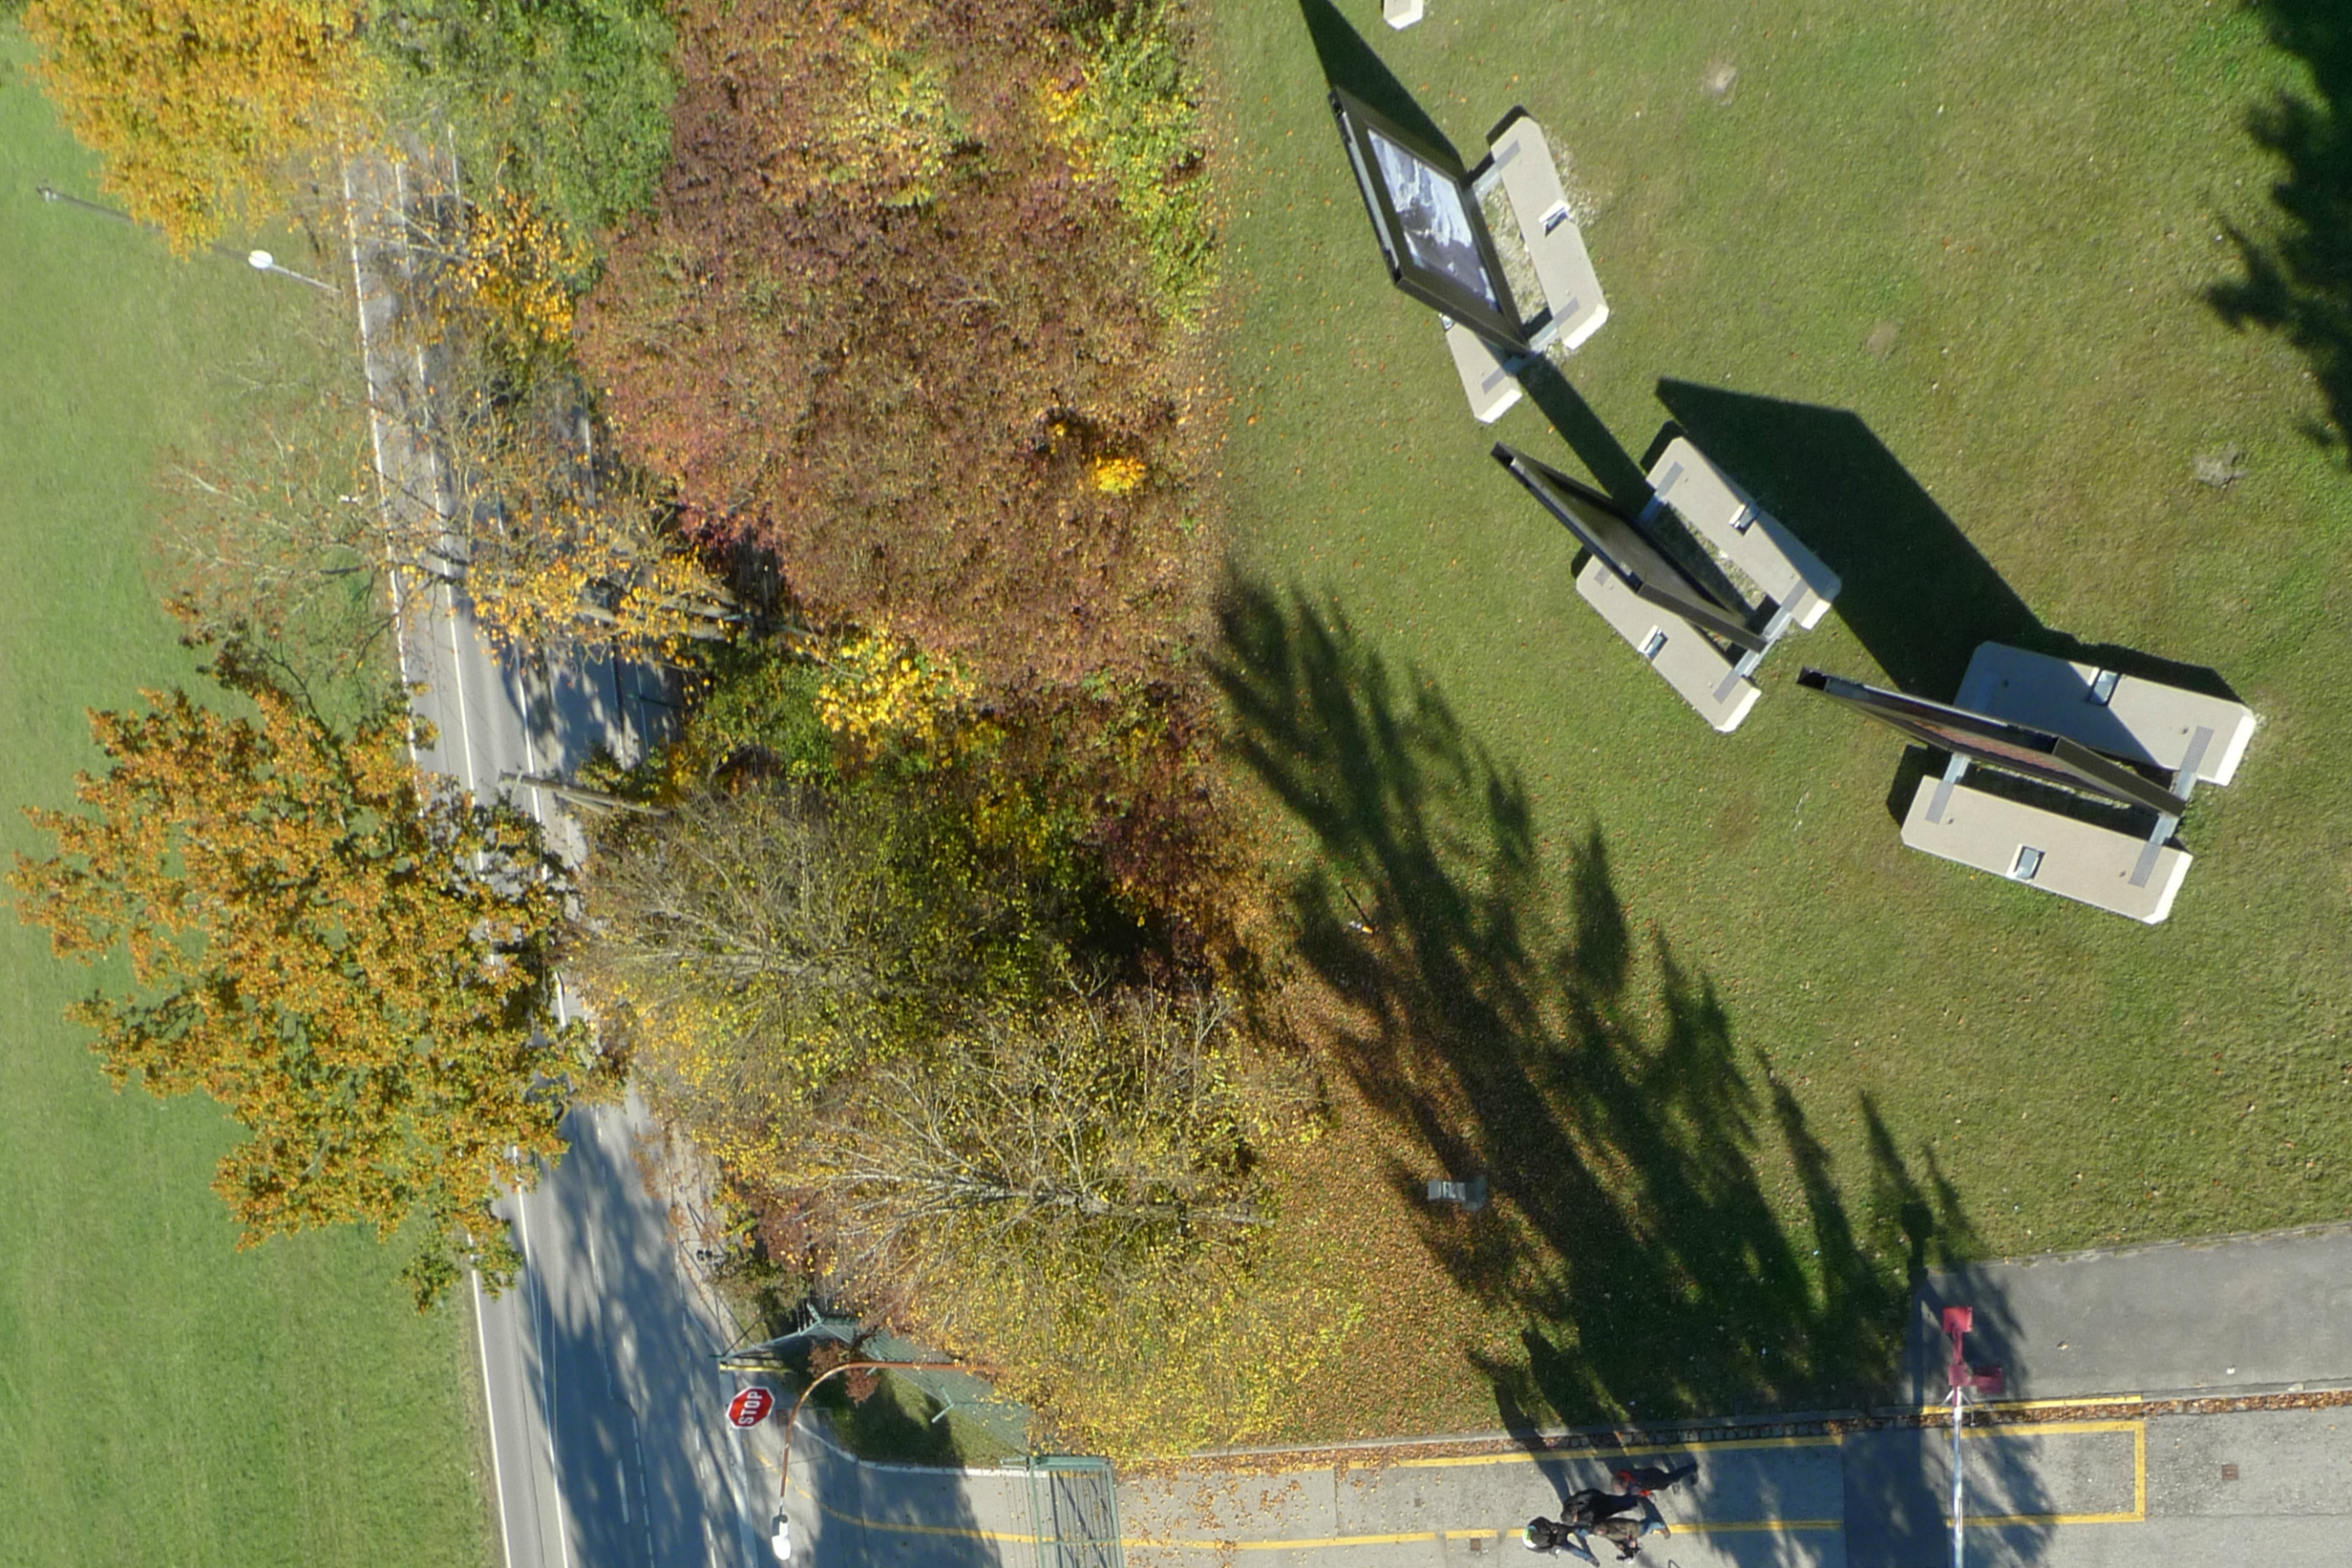
\includegraphics[cfbox=green,width=1\columnwidth]{P1110932}};    
 \end{tikzpicture}
 \end{subfigure}
\vspace{1.1\baselineskip}
\centerline{\textbf{(c)}}
 \caption{Comparison of UAV and aerial imagery. (a) aerial image, (b) magnified areas in aerial image, (c) UAV images featuring corresponding areas}
\end{figure}
 
On the other hand, the coverage of UAV imagery is of limited extent, therefore UAVs are typically used for small-scale mapping as an efficient alternative to full-scale aerial mapping. The total costs of UAV platforms are thus expected to be kept to a minimum, which is usually at the cost of the accuracy of onboard GNSS/IMU systems. Table \ref{tab:comp_acc} compares the accuracy and price of onboard GNSS/IMU systems for UAV and conventional airborne platforms

\begin{table}[H]
  \begin{center}
  %\footnotesize 
  \small
  \begin{tabular}{@{}p{.23\linewidth}p{.25\linewidth}p{.4\linewidth}@{}}
    \toprule
    {} & {\textbf{GNSS/IMU on UAV (NEO-M8)}} & {\textbf{GNSS/IMU on manned aircraft (xOEM)}} \\
    \cmidrule(){1-3}
    % %
    Horizontal accuracy & $2.5$ m & $0.02$ m \\
    \midrule
    Vertical accuracy & $5$ m & $0.03$ m \\
    \midrule
Heading accuracy& $0.3^{\circ}$  & $0.05^{\circ}\sim0.1^{\circ}$\\
    \midrule
    % %
    Price & $30$ \euro{} & $15000$ \euro{}\\ 
    \bottomrule
  \end{tabular}
  \end{center}
  \caption {Comparison of onboard GNSS/IMU systems for UAVs and conventional manned aircrafts}
\label{tab:comp_acc}
\end{table}

Drones are increasingly being used for surveying building construction, road maintenance, and infrastructure inspections. Agricultural applications include crop inspection, and tracking farm animals. 